\documentclass[12pt,a4paper]{article} 

\usepackage[russian]{babel}
\usepackage[T2A]{fontenc} 
\usepackage[utf8]{inputenc} 
\usepackage{graphicx}
\usepackage{amsmath}
\usepackage{amssymb}
\usepackage{amsfonts}
\usepackage{geometry}
\geometry{a4paper, total = {170mm, 257mm}, left = 20mm, top = 20mm}
\frenchspacing 

% counter
\newcounter{problem}
\renewcommand{\theproblem}{\arabic{problem}.}
\newcommand{\problem}{\refstepcounter{problem}\textbf{Задача~\theproblem~}}


\begin{document}
    \begin{center}
        {\textbf 
            {\Large
                Дифференциальная геометрия
                \\[2mm]
                ФН2-42Б, 2 курс, 4 семестр
                \\[10mm]
                Домашнее задание №1
                \\[2mm]
                <<Кривые и поверхности в пространстве>>
                \\[2mm]
                Вариант 2-23
            }
        }
    \end{center}

    \section*{Дано: }

    \hspace{5mm} Поверхность задана параметрически уравнениями $ S: \vec{\textbf r} = \vec{\textbf r}(u, v), \  u, v \in \mathbb{R} $

    Уравнение поверхности: 
    \[ \vec{\textbf r}(u, v) = \{ \cosh u \cos v,\ 5 \sinh u,\ \cosh u \sin v \} \]

    Вид кривой на поверхности и координаты точек: 
    \[ \gamma: u = v;\ P_1(1, 0, 0);\ P_2(-\cosh \pi, 5 \sinh \pi, 0) \]

    \section*{Задачи: }


    \hspace{7mm}\problem Найти особые точки параметризированной поверхности. Составить уравнение касательной к поверхности в точках $ P_1 $ и $ P_2 $
    
    \bigskip

    Для того, чтобы вывести уравнение касательной плоскости к поверхности в точке, необходимо найти вектор нормали к поверхности в точке. Сначала нужно взять частные производные $ \frac{\partial \vec{\textbf r}}{\partial u} = \vec{\textbf r}_u $ и $ \frac{\partial \vec{\textbf r}}{\partial v} = \vec{\textbf r}_v $: 

    \[
        \vec{\textbf r}_u = 
            \begin{pmatrix}
                \sinh u \cos v
                \\
                5\cosh u
                \\
                \sinh u \sin v
            \end{pmatrix};\  
        \vec{\textbf r}_v = 
            \begin{pmatrix}
                -\cosh u \sin v
                \\
                0
                \\
                \cosh u \cos v
            \end{pmatrix}
    \]

    Векторное произведение $ \vec{\textbf r}_u \times  \vec{\textbf r}_v $ имеет вид:

    \[
        \vec{\textbf r}_u \times  \vec{\textbf r}_v = 
            \begin{vmatrix}
                i && j && k
                \\
                \sinh u \cos v && 5\cosh u && \sinh u \sin v
                \\
                -\cosh u \sin v && 0 && \cosh u \cos v
            \end{vmatrix}
        =
    \]

    \bigskip

    \noindent $ = \vec{\textbf i}\,(5 \cosh^2 u \cos u ) + \vec{\textbf j}\,(\sinh u \cosh u \cos^2 - \sinh u \cosh u \sin^2 v) + \vec{\textbf k}\,(5 \cosh^2 u \sin v) $

    \[
        \vec{\textbf r}_u \times \vec{\textbf r}_v =
        \begin{pmatrix}
            5 \cosh^2 u \cos v
            \\
            -\sinh u \cosh u
            \\
            5 \cosh^2 u \sin v
        \end{pmatrix}
    \]

    Сразу можно заметить, что $ \vec{\textbf r}_u \times \vec{\textbf r}_v \ne \vec{\textbf 0}$ ни при каких значениях $ u \ \text{или} \ v $. Это означает, что все точки поверхности -- регулярные.

    \pagebreak

    Посчитаем норму векторного призведения $ | \vec{\textbf r}_u \times \vec{\textbf r}_v | $: 

    \[
        | \vec{\textbf r}_u \times \vec{\textbf r}_v | = \sqrt{25 \cosh^4 u + \sinh^2 y \cosh^2 u} = \cosh u \sqrt { 25 \cosh^2 u + \sinh^2 u } 
    \]

    Таким образом, вектор нормали $ \vec{\textbf n} $ имеет следующий вид: 
    
    \[
        \vec{\textbf n} = \frac{\vec{\textbf r}_u \times \vec{\textbf r}_v}{| \vec{\textbf r}_u \times \vec{\textbf r}_v |} = \frac{1}{\sqrt{25 \cosh^2 u + \sinh^2 u}}
        \begin{pmatrix}
            5 \cosh u \cos v
            \\
            -\sinh u
            \\
            5 \cosh u \sin v
        \end{pmatrix}
    \]

    Выразим координаты точек $ P_1 $ и $ P_2 $ через $ u \ \text{и} \ v $. Для этого приравняем координаты уравнения поверхности $ \vec{\textbf r}(u, v) $ к координатам этих точек:

    \[
        \begin{tabular}{lcl}
            $
                P_1: 
                \begin{cases}
                    \cosh u \cos v = 1
                    \\
                    5 \sinh u = 0
                    \\
                    \cosh u \sin v = 0
                \end{cases} 
            $ 
            & $ \Leftrightarrow $ & 
            $
                \begin{cases}
                    u_1 = 0
                    \\
                    v_1 = 0
                \end{cases}
            $

            \\ \\

            $
                P_2: 
                \begin{cases}
                    \cosh u \cos v = -\cosh \pi
                    \\
                    5 \sinh u =  5 \sinh \pi
                    \\
                    \cosh u \sin v = 0
                \end{cases}
            $ 
            & $ \Leftrightarrow $ & 
            $
                \begin{cases}
                    u_2 = \pi
                    \\
                    v_2 = \pi
                \end{cases}
            $

        \end{tabular}
    \]

    Теперь мы можем вычислить нормали касательных плоскостей в точках $ P_1 $ и $ P_2 $ соответсвенно. 
    
    В точке $ {P_1} $ вектор единичной нормали равен:

    \[
        \vec{\textbf n}|_{P_1} =
        \begin{pmatrix}
            1 
            \\ 
            0 
            \\ 
            0  
        \end{pmatrix},
    \]

    \noindent тогда касательная плоскость имеет вид: 

    \[
        T_{P_1}: x - 1 = 0
    \]


    В точке $ {P_2} $ вектор единичной нормали равен:

    \[
        \vec{\textbf n}|_{P_2} = \frac{1}{\sqrt{25 \cosh^2 \pi + \sinh^2 \pi}}
        \begin{pmatrix}
            -5 \cosh \pi
            \\
            -\sinh \pi
            \\
            0
        \end{pmatrix}, 
    \]

    \noindent и касательная плоскость имеет вид: 

    \[
        T_{P_2}: 5 \cosh \pi \cdot x + \sinh \pi \cdot y + 5 = 0
    \]

    \bigskip

    \begin{flushright}
        \begin{tabular}{rl}
            \textbf{Ответ:} & Особых точек нет;

            \\

                            & $ T_{P_1}: x - 1 = 0 $;

            \\

                            & $ T_{P_2}: 5 \cosh \pi \cdot x + \sinh \pi \cdot y + 5 = 0 $.
        \end{tabular}
    \end{flushright}

    \pagebreak

    \problem Исследовать зависимость вида поверхности от области изменения параметров $ (u, v) $. Составить уравнения координатных линий. Построить поверхность и координатную сеть на ней (с использованием системы компьютерной алгебры Wolfram Mathematica)

    \bigskip
    
    Уравнение поверхности, выраженное через $ x, y, z $: 

    \[
        \begin{cases}
            x = \cosh u \cos v
            \\
            y = 5 \sinh u
            \\
            z = \cosh u \sin v
        \end{cases} 
        \Leftrightarrow \ 
        x^2 + z^2 - \frac{y^2}{25} = 1, 
    \]

    \noindent значит, данная поверхность -- однополостный гиперболоид с осью вдоль $ OY $

    \begin{figure}[!h]
        \centering
        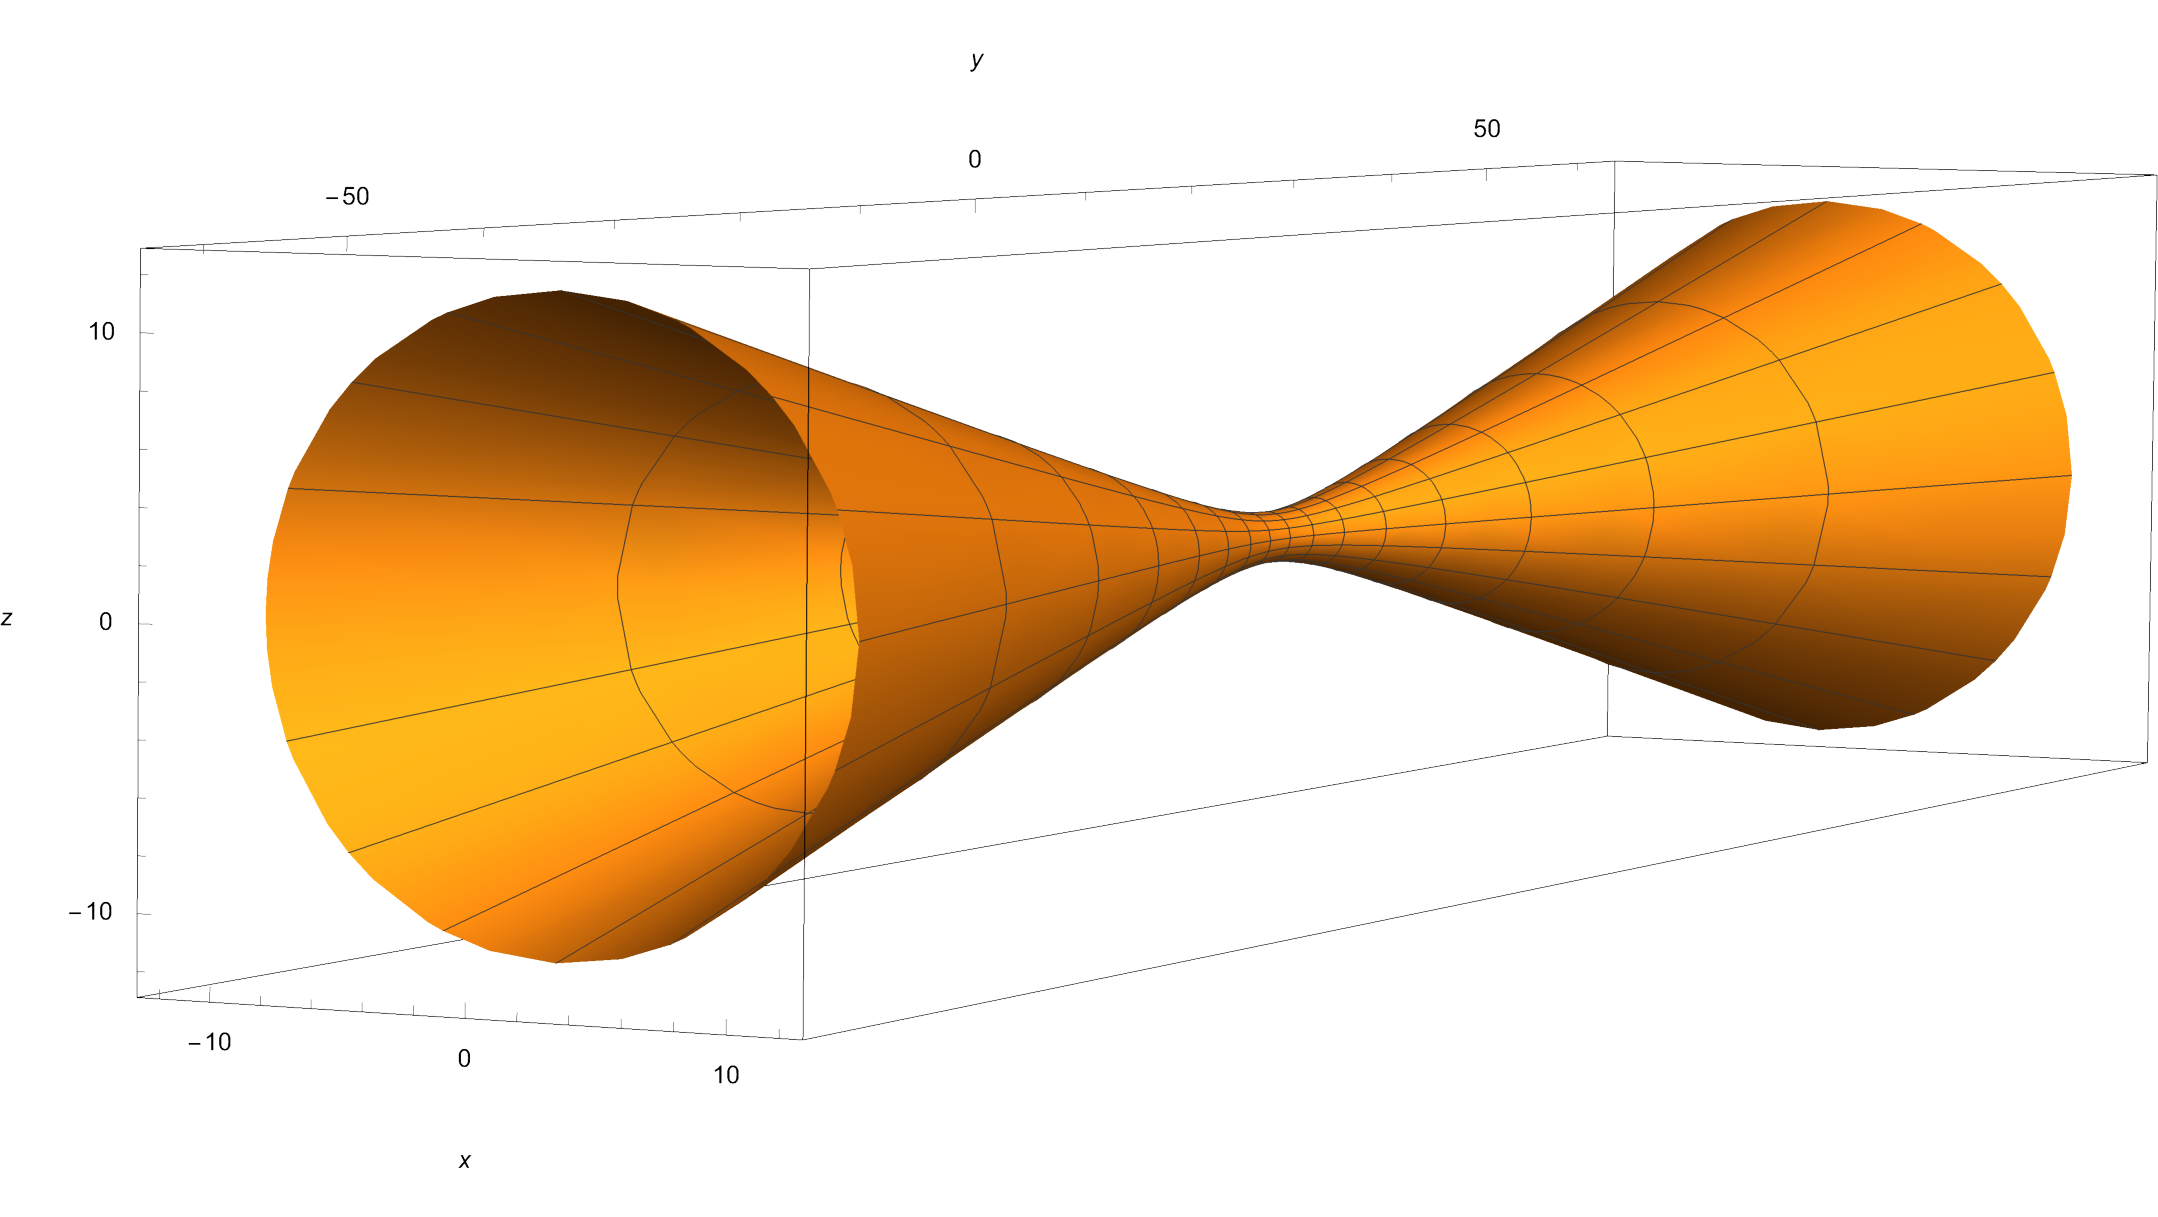
\includegraphics[width=0.8\textwidth]{Hyp.pdf}
        \caption{Однополостный гиперболоид}
        \label{fig:hyp}
    \end{figure}

\end{document}